\chapter{一类电报方程的辛方法研究}
\echapter{Study on Symplectic Method for Telegraph Equations}

本章介绍一类含有齐次初边值条件电报方程的辛方法,该方法的思想是利用一个特殊的变换,把不具有守恒性的电报方程,变为具有守恒性质的 Klein-Gordon 方程进行求解.对于变换后的守恒结构,我们结合辛方法进行求解.

传输线主要用来传输无线电频率的交变电流,反映了当电流频率高到一定程度时的波的性质.传输线广泛应用在信号传输,产生脉冲和信号过滤等领域.常见的传输线主要有平行线、同轴电缆、
带状线、微带线、波导管、介质波导和光纤,等等.电报方程,也称为传输线方程或电报员方程,来源于Maxwell方程组,是描述传输线里电流电压属性的一类方程.更具体地讲,电报方程来源于这样的问题,导体由无限个二端口元件连接而成,每一个元件都是很小的传输线元件.一般的传输线方程可以由图~\ref{fig:tele1} 中的等效模型,其关系可根据基尔霍夫电压和电流定律导出~\cite{ludwig2000rf}.

现有的关于求解电报方程的方法通常分为两大类,第一类是求精确解,第二类是求数值解.精确解只对一小部分方程有效,其他问题还需要用数值模拟来解决.求数值解的方法,从思想上可以分为两种,第一种是用解析的方法,将解的波形迭代起来求解,第二种则是离散方程之后的数值计算,即离散求解.解析方法通过迭代波形,使得结果逐渐逼近真解.常见的解析方法有 Exp-函数方法~\cite{naher2011exp}, Adomian 分解方法~(ADM)~\cite{adomian1988areview,sheikholeslami2012analytical}, 变分迭代方法~(VIM)~\cite{wu2013variational} 和同伦摄动方法~(HPM)~\cite{sheikholeslami2012homotopy}. 电报方程的离散方法常见的有微分二次方法~(DQM)~\cite{jiwari2012numerical}, 交替迭代隐式方法~(ADI) \cite{cui2013convergence}, 和 WENO 方法 \cite{borges2008improved,shen2014improvement}.

这里简要介绍各种解析方法的思想. Exp-函数方法是利用行波变换将偏微分方程转换为常微分方程,然后再将常微分方程的解用指数函数展成分式形式,过程中产生了一些待定常数,最后求解待定常数. Adomian 分解方法由 George Adomian 提出,该方法将算子的线性部分和非线性部分分裂开来,再设计迭代格式,是一种逼近真解的解析方法.变分迭代方法是一种迭代方法,主要有三个步骤,构造修正泛函,构造 Lagrange 乘子,确定初始迭代,其中第二步的构造 Lagrange 乘子是最重要的也是最困难的.同伦摄动方法和 Adomian 分解方法开始的步骤类似,将算子的线性部分和非线性部分分裂开来,然后再利用摄动方法,构造一个同伦,摄动的极限就是方程的真解.

常用的离散方法的基本思想如下.微分二次方法是把方程的每一项,包括函数值,及其各阶偏导数值,对于一组特殊的基进行展开,最后确定展开的系数,其衍生的方法有多项式微分二次方法等等.交替迭代隐式方法作为一种隐式差分数值格式,在高维问题的计算中有着较为好的效果,主要擅长计算热传导和扩散类方程.其思想是将一个有限差分格式沿着不同的空间方向分裂成两步,再进行计算.其优点是无条件稳定且时间空间二阶,也有更高阶的格式可以构造. WENO 方法是基于 ENO 方法提出来的,擅长于求解双曲型问题,比如交通流问题,波动类方程,等等.该方法是一种加权求值方法,通过特殊的构造权值,对 ENO 方法进行了改进,该方法对于分片光滑问题有着较好的效果.

本章所研究的是这样一类电报方程
\begin{equation}\label{eq:tele}
\left\lbrace
\begin{aligned}
&\frac{\partial ^2 w(x,t)}{\partial t^2}+k\frac{\partial w(x,t)}{\partial t}=a^2 \frac{\partial ^2 w(x,t)}{\partial x^2} + b w(x,t),\\
&\begin{aligned}
w(x,0)&=g_1(x),&0 \le x \le 1,\\
w_t(x,0)&=g_2(x),&0 \le x \le 1,\\
w(0,t)&=0,&0 \le t \le T,\\
w(1,t)&=0,&0 \le t \le T,
\end{aligned}
\end{aligned}
\right.
\end{equation}
式中 $k > 0$, $a>0$ 和 $b < 0$ 是常数. $g_1(x)$ 和 $g_2(x)$ 是光滑函数, 满足相容性条件 $g_1(0)=0$. $w(x,t) \in \mathbb{R}$ 为所求函数. 此方程对应于如下的一类传输线方程,方程的等效电路图如图~\ref{fig:tele1}. 图中,要求 $a^2 = \frac{1}{L_1C_1}, k= (\frac{R_2^{-1}}{C_1}+\frac{R_1}{L_1}), b =-\frac{R_1R_2^{-1}}{L_1C_1}$.
\begin{figure}[h]
    \centering
    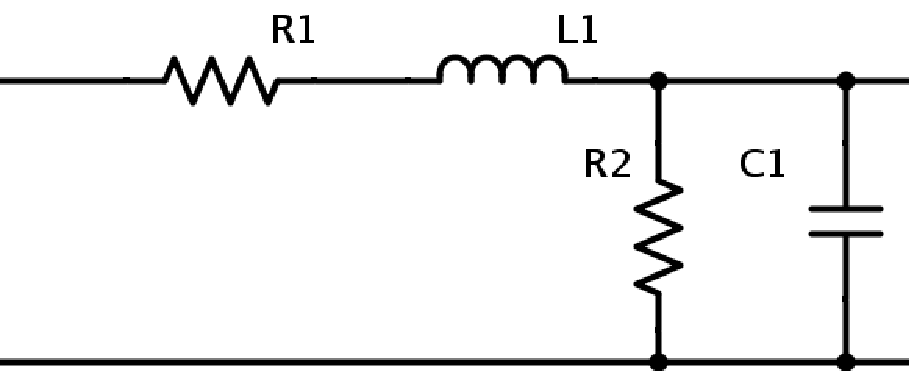
\includegraphics[width=0.5\textwidth]{02/Fig1.pdf}
    \caption{传输线方程的等效电路图}
    \label{fig:tele1}
\end{figure}

在本章中,我们针对具有齐次边界条件的电报方程 \eqref{eq:tele} 进行求解.该求解方法适用于一维和高维问题.本章的基本框架如下.首先在 \ref{sec:02symplectic} 中介绍辛方法.接下来,在 \ref{sec:02telegraph} 中逐步展开介绍我们的方法及其相关理论,数值结果将在 \ref{sec:02numerical} 中给出.最后一部分 \ref{sec:02conclusion} 是小结.

\section{辛的基本概念}\label{sec:02symplectic}
\esection{Introduction to the Symplectic Method}
辛方法 \cite{feng2010symplectic} 是求解较长时间区间的哈密尔顿系统的行之有效的方法.用辛方法求解哈密尔顿系统的做法给予人们新的启迪,指引着人们去寻找好的优美的方法.辛方法起源于 de Vogelaere (1956), Ruth (1983)和 冯康 (1985) 的工作 \cite{hairer2006geometric}, 其基本思想是避开盲目对精度的苛求,巧妙地利用哈密尔顿系统的辛结构,改为保持该结构作为目标,构造数值格式.理论和数值算例都验证了该方法的优越性,系统的数值能量能够保持在系统的真实值附近波动.数十年来,辛方法迅速发展起来,并且得到了不断地发扬光大 \cite{calvo1994numerical,leimkuhler2004simulating,hong2006multi,yang2009extended,monovasilis2013exponentially,xin2016birkhoffian,michalas2016numerical,liao2016multi}. 该方法数值算例证实了辛数值积分格式比非辛格式的优越性.因此,在处理多体问题和其他哈密尔顿系统问题上,有着较好的应用.

哈密尔顿系统是由数学家 Hamilton 构造出来,用来描述物理系统的发展型方程.该表示的优点是能够在无法求得该系统的解析解的情况下,阐明一些动力系统的性态.在工程应用中, 包括动力学、分子动力学、流体力学、量子力学、图像处理、天体力学、核工程等领域在内的问题,都可以表示成如下的哈密尔顿系统的形式 \cite{arieh2009afirst}
\begin{equation}\label{eq:Hamiltonian}
\left\lbrace
\begin{aligned}
\frac{dq}{dt}&=\frac{\partial H}{\partial p},\\
\frac{dp}{dt}&=-\frac{\partial H}{\partial q},
\end{aligned}
\right.
\end{equation}
式中 $p \in \mathbb{R}^d$ 和 $q \in \mathbb{R}^d$ 为所求函数, $H=H(q,p)$ 是系统的哈密尔顿量.在实际应用中, $d$ 为该哈密尔顿系统的自由度, $q$ 与 $p$ 分别对应系统的广义位移和广义动量.在相空间 $\mathbb{R}^{2d}$ 上的标准辛形式是如下的二微分形式
\begin{equation*}
\omega = \sum_{i=1}^d d q_i \wedge d p_i.
\end{equation*}
保持哈密尔顿系统辛结构的数值方法称之为辛方法,在后面部分会给出准确的定义.常用的辛方法有隐式中点法,交错显式格式,基于 Pad\'{e} 逼近的方法, St\"{o}rmer-Verlet 格式,辛 Runge-Kutta 方法,等等.

在本小节,我们列出了几种具有代表性的辛格式.哈密尔顿系统具有一个守恒的哈密尔顿量 $H(q,p)$, 其中 $q$ 表示位移 $p$ 表示动量.


令 $\Phi_h : \mathbb{R}^{2d} \to \mathbb{R}^{2d}$ 表示时间步进的数值算法进行一步计算的函数, 其中 $d$ 为 $p$ 和 $q$ 的维数. $z_{n+1}=\Phi_h(z_n)$ 其中 $z_n$ 是在第 $n$ 步时间点上数值解.辛方法则是具有以下性质的一类方法.

\begin{definition}[辛方法~\cite{hairer2006geometric}]
\emph{一个单步的数值方法 $z_{n+1}=\Phi_h(z_n)$ 称为辛方法,如果该方法保持二形式
\begin{equation*}
dq_{n+1}\wedge dp_{n+1}=dq_n\wedge dp_n,
\end{equation*}
式中 $z_n=(q_n,p_n)^T,~n=1,2,\cdots$.}
\end{definition}

下面是辛方法的一个等价定义.

\begin{definition}[辛方法~\cite{hairer2006geometric}]\label{def:symplectic}
\emph{一个单步的数值方法 $z_{n+1}=\Phi_h(z_n)$ 称之为辛方法,如果 $\Phi_h$ 的 Jacobian 矩阵满足
\begin{equation*}
(\nabla\Phi_h)^TJ^{-1}(\nabla\Phi_h)=J^{-1}.
\end{equation*}}
\end{definition}

\begin{remark}
{\rm 定义 \ref{def:symplectic} 使得我们能够更容易验证数值格式的辛性质.为了获得更多的,更高阶的辛方法,需要使用生成函数法,见 \cite{hairer2006geometric}.}
\end{remark}

接下来,在这里给出一些辛方法的例子.

\noindent \textbf{隐式中点法}
\begin{equation*}
\frac{z^{n+1}-z^n}{\tau}=J^{-1}H_z(\frac{z^{n+1}+z^n}{2}),
\end{equation*}
为二阶辛方法.

\noindent \textbf{辛欧拉法}
\begin{equation*}
\begin{aligned}
p_{n+1}&=p_n-hH_q(p_{n+1},q_n),\\
q_{n+1}&=q_n+hH_p(p_{n+1},q_n),
\end{aligned}
\quad \text{or} \quad
\begin{aligned}
p_{n+1}&=p_n-hH_q(p_n,q_{n+1}),\\
q_{n+1}&=q_n+hH_p(p_n,q_{n+1}),
\end{aligned}
\end{equation*}
均为一阶方法.

\noindent \textbf{St\"{o}rmer-Verlet 格式}
\begin{equation*}
\begin{aligned}
p_{n+1/2}&=p_n-\frac{h}{2}H_q(p_{n+1/2},q_n),\\
q_{n+1}&=q_n+\frac{h}{2}(H_p(p_{n+1/2},q_n)+H_p(p_{n+1/2},q_{n+1})),\\
p_{n+1}&=p_{n+1/2}-\frac{h}{2}H_q(p_{n+1/2},q_{n+1}),
\end{aligned}
\end{equation*}
和
\begin{equation*}
\begin{aligned}
q_{n+1/2}&=q_n+\frac{h}{2}H_q(p_n,q_{n+1/2}),\\
p_{n+1}&=p_n-\frac{h}{2}(H_p(p_n,q_{n+1/2})+H_p(p_{n+1},q_{n+1/2})),\\
q_{n+1}&=q_{n+1/2}+\frac{h}{2}H_q(p_{n+1},q_{n+1/2}),
\end{aligned}
\end{equation*}
均为二阶方法.

\noindent \textbf{辛 Runge-Kutta 方法}

对于 Runge-Kutta 方法,我们知道, $\nu$ 步的 Runge-Kutta 方法可以写成
\begin{equation*}
  \left\lbrace
    \begin{aligned}
      Y_{n+1}^{r}&=\eta(t_{n})+h\sum_{s=1}^{\nu}a_{rs}f(t_{n+1}^{s},Y_{n+1}^{s}),\quad r=1,\cdots, \nu, \\
      \eta(t_{n+1})&=\eta(t_{n})+h\sum_{s=1}^{\nu}b_{s}f(t_{n+1}^{s},Y_{n+1}^{s}).
    \end{aligned}
  \right.
\end{equation*}

其对应的 Butcher 表可以写成

\begin{center}
  \begin{tabular}{c|cccc}
    $c_1$&$a_{11}$&$a_{12}$&$\cdots$&$a_{1\nu}$\\
    $c_2$&$a_{21}$&$a_{22}$&$\cdots$&$a_{2\nu}$\\
    $\vdots$&$\vdots$&$\vdots$&$\ddots$&$\vdots$\\
    $c_{\nu}$&$a_{\nu 1}$&$a_{\nu 2}$&$\cdots$&$a_{\nu \nu}$\\
    \hline
         &$b_{1}$&$b_{2}$&$\cdots$&$b_{\nu}$
  \end{tabular}
\end{center}

\begin{theorem}{辛 Runge-Kutta 方法\cite{sanz1988runge}}
\emph{如果该 Runge-Kutta 的 Butcher 表满足
\begin{equation*}
  b_ia_{ij}+b_ja_{ji}=b_ib_j,\quad \textrm{对所有}\,\, i,j=1,2,\cdots,\nu,
\end{equation*}
则该 Runge-Kutta 方法是保辛的.}
\end{theorem}

对于辛 Runge-Kutta 方法,它的阶数和对应的 Runge-Kutta 方法的阶数相同,可以用根树理论和B级数理论来求得.

\noindent \textbf{由生成函数构造的辛方法}

根据生成函数的构造理论,能够得到一系列如下的辛格式 \cite{feng2003sym}.

$1$ 阶格式

\begin{equation*}
	p_i^{k+1}= p_i^{k}-hH_{q_i}(p^{k+1},q^{k}),
\end{equation*}
\begin{equation*}
	q_i^{k+1}= q_i^{k}+hH_{p_i}(p^{k+1},q^{k}),
\end{equation*}
式中 $i=1,\ldots,n$.

$2$ 阶格式

\begin{equation*}
	p_i^{k+1}= p_i^{k}-hH_{q_i}(p^{k+1},q^{k})-\frac{h^2}{2}\sum_{j=1}^n(H_{q_j}H_{p_j})_{q_i}(p^{k+1},q^{k}),
\end{equation*}
\begin{equation*}
	q_i^{k+1}= q_i^{k}+hH_{p_i}(p^{k+1},q^{k})+\frac{h^2}{2}\sum_{j=1}^n(H_{q_j}H_{p_j})_{p_i}(p^{k+1},q^{k}),
\end{equation*}
式中 $i=1,\ldots,n$.

$3$ 阶格式

\begin{equation*}
\begin{aligned}
	p_i^{k+1}= &p_i^{k}-hH_{q_i}(p^{k+1},q^{k})-\frac{h^2}{2}\sum_{j=1}^n(H_{q_j}H_{p_j})_{q_i}(p^{k+1},q^{k})\\
	&-\frac{h^3}{6}\sum_{i,j=1}^n(H_{p_lp_j}H_{q_l}H_{q_j}+H_{q_lq_j}H_{p_l}H_{p_j}+H_{p_lq_j}H_{q_l}H_{p_j})_{q_i}(p^{k+1},q^{k}),
\end{aligned}
\end{equation*}
\begin{equation*}
\begin{aligned}
	q_i^{k+1}= &q_i^{k}+hH_{p_i}(p^{k+1},q^{k})+\frac{h^2}{2}\sum_{j=1}^n(H_{q_j}H_{p_j})_{p_i}(p^{k+1},q^{k})\\
	&+\frac{h^3}{6}\sum_{i,j=1}^n(H_{p_lp_j}H_{q_l}H_{q_j}+H_{q_lq_j}H_{p_l}H_{p_j}+H_{p_lq_j}H_{q_l}H_{p_j})_{p_i}(p^{k+1},q^{k}),
\end{aligned}
\end{equation*}
式中 $i=1,\ldots,n$.

\noindent \textbf{可分系统的多级显式方法}

对于可分的哈密尔顿系统, $H(q,p)=V(q)+U(p)$, 该系统可以写成
\begin{equation*}
	\frac{d}{dt}\begin{bmatrix}
	q\\
	p
	\end{bmatrix}=\begin{bmatrix}
	g(p)\\
	f(q)
	\end{bmatrix},
\end{equation*}
有如下一系列的多级显式格式 \cite{qin2011struc}.

$1$阶精度$1$级辛格式
\begin{equation*}
	p^{k+1}=p^{k}+hc_1f(q^{k}),\quad q^{k+1}=q^{k}+hd_1g(p^{k+1}),
\end{equation*}
式中 $c_1=d_1=1$.

$2$阶精度$2$级辛格式
\begin{equation*}
	\left\lbrace \begin{aligned}
		&p_1=p^{k}+hc_1f(q^{k}),\quad q_1=q^{k}+hd_1g(p_1),\\
		&p^{k+1}=p_1+hc_2f(q_1),\quad q^{k+1}=q_1+hd_2g(p^{k+1}),
	\end{aligned}\right.
\end{equation*}
式中 $c_1=0,c_2=1,d_1=d_2=\frac{1}{2}$ 或$d_1=1,d_2=0,c_1=c_2=\frac{1}{2}$.

$3$阶精度$3$级辛格式
\begin{equation*}
	\left\lbrace \begin{aligned}
		&p_1=p^{k}+hc_1f(q^{k}),\quad q_1=q^{k}+hd_1g(p_1),\\
		&p_2=p_1+hc_2f(q_1),\quad q_2=q_1+hd_2g(p_2),\\
		&p^{k+1}=p_2+hc_3f(q_2),\quad q^{k+1}=q_2+hd_3g(p^{k+1}),
	\end{aligned}\right.
\end{equation*}
式中
\begin{equation*}
	c_1=\frac{7}{24},\quad c_2=\frac{3}{4},\quad c_3=-\frac{1}{24},
\end{equation*}
\begin{equation*}
	d_1=\frac{2}{3},\quad d_2=-\frac{2}{3},\quad d_3=1,
\end{equation*}
或
\begin{equation*}
	c_1=1,\quad c_2=-\frac{2}{3},\quad c_3=\frac{2}{3},
\end{equation*}
\begin{equation*}
	d_1=-\frac{1}{24},\quad d_2=\frac{3}{4},\quad d_3=\frac{7}{24}.
\end{equation*}

$4$阶精度$4$级辛格式
\begin{equation*}
	\left\lbrace \begin{aligned}
		&p_1=p^{k}+hc_1f(q^{k}),\quad q_1=q^{k}+hd_1g(p_1),\\
		&p_2=p_1+hc_2f(q_1),\quad q_2=q_1+hd_2g(p_2),\\
		&p_3=p_2+hc_2f(q_2),\quad q_3=q_2+hd_2g(p_3),\\
		&p^{k+1}=p_3+hc_3f(q_3),\quad q^{k+1}=q_3+hd_4g(p^{k+1}),
	\end{aligned}\right.
\end{equation*}
式中
\begin{equation*}
	c_1=0,\quad c_2=c_4=\frac{1}{2}(2+\alpha),\quad c_3=-\frac{1}{4}(1+2\alpha),
\end{equation*}
\begin{equation*}
	d_1=d_4=\frac{1}{6}(2+\alpha),\quad d_2=d_3=\frac{1}{6}(1-\alpha),
\end{equation*}
或
\begin{equation*}
	c_1=\frac{1}{6}(2+\alpha),\quad c_2=c_3=\frac{1}{6}(1-\alpha),\quad c_4=\frac{1}{2}(2+\alpha),
\end{equation*}
\begin{equation*}
	d_1=\frac{1}{3}(2+\alpha),\quad d_2=-\frac{1}{3}(1+2\alpha),\quad d_3=\frac{1}{2}(2+\alpha),\quad d_4=0,
\end{equation*}
这里 $\alpha = 2^{\frac{1}{3}}+2^{-\frac{1}{3}}$.

\noindent \textbf{多级隐式辛方法}

这里举几个多级隐式辛格式 \cite{qin2011struc}
\begin{equation*}
	\left\lbrace \begin{aligned}
		&z^{k+1}=2Y_1-z^k,\\
		&Y_1=z^k+\frac{1}{2}hSY_1,
	\end{aligned}\right.
\end{equation*}

\begin{equation*}
	\left\lbrace \begin{aligned}
		&z^{k+1}=2Y_2-(2Y_1-z^k),\\
		&Y_1=z^k+\frac{1}{4}hSY_1,\\
		&Y_2=2Y_1-z^k+\frac{1}{4}hSY_2,
	\end{aligned}\right.
\end{equation*}

\begin{equation*}
	\left\lbrace \begin{aligned}
		&z^{k+1}=2Y_3-(2Y_2-2Y_1+z^k),\\
		&Y_1=z^k+\frac{1}{2}ahSY_1,\\
		&Y_2=2Y_1-z^k+\frac{1}{2}ahSY_2,\\
		&Y_3=2Y_2-(2Y_1-z^k)+(\frac{1}{2}-a)hSY_3,
	\end{aligned}\right.
\end{equation*}

\begin{equation*}
	\left\lbrace \begin{aligned}
		&z^{k+1}=2Y_4-(2Y_3-2Y_2+2Y_1-z^k),\\
		&Y_1=z^k+\frac{1}{2}b_1hSY_1,\\
		&Y_2=2Y_1-z^k+\frac{1}{2}b_2hSY_2,\\
		&Y_3=2Y_2-(2Y_1-z^k)+\frac{1}{2}b_3hSY_3,\\
		&Y_4=2Y_3-(2Y_2-2Y_1+z^k)+\frac{1}{2}b_4hSY_4,
	\end{aligned}\right.
\end{equation*}
式中 $a=1.351207,~ b_1=-2,703094,~ b_2=-0.536527,~ b_3=1.860681$.

令
\begin{equation*}
	S=\begin{bmatrix}
		0&M_1\\
		I&0
	\end{bmatrix}\quad \text{或} \quad S=\begin{bmatrix}
		0&M_3\\
		M_3&0
	\end{bmatrix},
\end{equation*}
则上面的格式依次有精度 $o(\Delta t+\Delta x^2),~o(\Delta t+\Delta x^2),~o(\Delta t^3+\Delta x^2),~o(\Delta t^4+\Delta x^2)$.

若取
\begin{equation*}
	S=\begin{bmatrix}
		0&M_2\\
		I&0
	\end{bmatrix}\quad \text{或} \quad S=\begin{bmatrix}
		0&M_4\\
		M_4&0
	\end{bmatrix},
\end{equation*}
则上面的格式依次有精度 $o(\Delta t+\Delta x^4),~o(\Delta t^t+\Delta x^4),~o(\Delta t^3+\Delta x^4),~o(\Delta t^4+\Delta x^4)$.
这里
\begin{equation*}
	M_1=\frac{1}{\Delta x^2}\begin{bmatrix}
		-2&1&0&\cdots&\cdots&1\\
		1&-2&1&\cdots&\cdots&0\\
		&\ddots&\ddots&\ddots&&\\
		&&\ddots&\ddots&\ddots&\\
		0&0&\cdots&\cdots&-2&1\\
		1&0&\cdots&\cdots&1&-2
	\end{bmatrix},\quad M_3=\frac{1}{2\Delta x}\begin{bmatrix}
		0&1&0&\cdots&\cdots&-1\\
		-1&0&1&\cdots&\cdots&0\\
		&\ddots&\ddots&\ddots&&\\
		&&\ddots&\ddots&\ddots&\\
		0&0&\cdots&\cdots&0&1\\
		1&0&\cdots&\cdots&-1&0
	\end{bmatrix},
\end{equation*}
\begin{equation*}
	M_2=\frac{1}{12\Delta x^2}\begin{bmatrix}
-30 & 16 & -1 & 0 & 0 & \cdots & \cdots & 0 & -1 & 16 \\
16 & -30 & 16 & -1 & 0 & \cdots & \cdots & 0 & 0 & -1 \\
-1 & 16 & -30 & 16 & -1 & \cdots & \cdots & 0 & 0 & 0 \\
\ddots & \ddots & \ddots & \ddots &   &   &   &   &   &   \\
&\ddots & \ddots & \ddots & \ddots &   &   &   &   &\\
&&\ddots & \ddots & \ddots & \ddots &   &   &   &-1\\
&&&\ddots & \ddots & \ddots & \ddots &   &   &-1\\
-1 & 0 & 0 & \cdots & \cdots & \cdots & -1 & 16 & -30 & 16 \\
16 & -1 & 0 & \cdots & \cdots & \cdots & 0 & -1 & 16 & -30
\end{bmatrix},
\end{equation*}
\begin{equation*}
	M_4=\frac{1}{12\Delta x}\begin{bmatrix}
0 & 8 & -1 & 0 & 0 & \cdots & \cdots & \cdots & 1 & -8\\
-8 & 0 & 8 & -1 & 0 & \cdots & \cdots & \cdots & 0 & 1\\
1 & -8 & 0 & 8 & -1 & \cdots & \cdots & \cdots && \\
\ddots & \ddots & \ddots & \ddots &   &   &   &   && \\
&\ddots & \ddots & \ddots & \ddots &   &   &   &&\\
&&\ddots & \ddots & \ddots & \ddots &   &   && \\
-1 & 0 & 0 & \cdots & \cdots & \cdots & 1 & -8 & 0&8 \\
8&-1 & 0 & 0 & \cdots  & \cdots & \cdots & 1 & -8 & 0
\end{bmatrix}.
\end{equation*}

辛方法是一大类方法的总称,其延伸及其推广包括辛 Runge-Kutta 法 \cite{feng2010symplectic,burrage2014structure}, 辛 RKN 方法 \cite{monovasilis2013exponentially}, 辛 ERKN 方法 \cite{yang2009extended}, 等等.这些方法中一部分为隐式方法,另外,辛 Runge-Kutta 方法均为隐式方法 \cite{sanz1988runge}.

\section{电报方程的辛方法}\label{sec:02telegraph}
\esection{Symplectic Methods for Telegraph Equations}

电报方程的系统能量随时间而指数衰减.经过研究,发现了这样一个变换,能够使电报方程 \eqref{eq:tele} 变为一个守恒的系统,而这种守恒性刚好能让方程利用辛方法进行求解.这样做带来的好处是能够有效地求解更长的时间区间,获得更容易实现的数值格式.我们将在 \ref{sec:02transform} 节中详细介绍这种变换.

方程 \eqref{eq:tele} 的差分格式通常可以从两个角度来入手.一种是全离散,也就是说,对空间和时间进行等间距的网格的划分 $x_0=0<x_1<\cdots<x_N=1,~t_0=0<t_1<\cdots<t_n=T$. 之后,能够得到全离散的结果
\begin{equation}\label{eq:fulld}
\frac{w_{i}^{j+1}-2w_{i}^{j}+w_{i}^{j-1}}{\Delta t^2}+k\frac{w_{i}^{j+1}-w_{i}^{j}}{\Delta t}=a^2
\frac{w_{i+1}^{j+1}-2w_{i}^{j+1}+w_{i-1}^{j+1}}{\Delta x^2} + b w_{i}^{j+1},
\end{equation}
式中, $1 \le i \le N-1$ 和 $1 \le j \le n-1$. 式 $w_{i}^{j}$ 分别是在空间和时间格点上的数值,即$w(x_i,t_j)=w_{i}^{j}$.
另外一种则是半离散.如果取等间距的空间网格划分 $x_0=0<x_1<\cdots<x_N=1$, 将得到一个常微分方程组 (ODEs),
\begin{equation*}
\frac{d^2 W_i}{d t^2}+k\frac{d W_i}{d t}=a^2 \frac{W_{i+1}-2W_{i}+W_{i-1}}{\Delta x^2} + b W_i,
\end{equation*}
式中, $1 \le i \le N-1$, 和 $W_i = W(x_i,t)$. 这里,我们采用了时间二阶离散.

令 $W=(W_1,W_2,\cdots,W_{N-1})^T$, 则有
\begin{equation}\label{eq:fd}
\frac{d^2 W}{d t^2}+k\frac{d W}{d t}= -\frac{a^2}{\Delta x^2}SW + b W,
\end{equation}
式中
\begin{equation}\label{eq:s}
S=\begin{pmatrix}
2&-1&&&\\
-1&2&1&&\\
&-1&2&\ddots&\\
&&\ddots&\ddots&-1\\
&&&1&2
\end{pmatrix}.
\end{equation}

为了获得稳定的数值格式,在用差分方法求解方程 \eqref{eq:fd} 的时候,在时间离散上通常采用隐式格式.注意到如果方程 \eqref{eq:tele} 的边界条件适当,则可以将方程 \eqref{eq:fd} 写成哈密尔顿系统的形式.在此条件下,对方程 \eqref{eq:tele} 做一个变换,利用这个变换把方程 \eqref{eq:fd} 中的阻尼项 $k\frac{d W}{d t}$ 去掉.该变换能把一个电报方程变换成 Klein-Gordon 方程,因此能够得到更加容易求解的哈密尔顿系统.

接下来,针对一维和高维两种情况来介绍我们的算法 \ref{alg:tele}. 算法基本分三个步骤,即做变换,离散求解哈密尔顿系统,做逆变换得到数值解.

\begin{algorithm}
\caption{电报方程求解基本算法}
\begin{algorithmic}[1]
\STATE 将电报方程 \eqref{eq:tele} 变换成相应的 Klein-Gordon 方程. 相应地改变初边值条件. \newline
\STATE 离散得到的 Klein-Gordon 方程成为哈密尔顿方程组. 使用辛方法求解该哈密尔顿系统,得到 Klein-Gordon 方程的数值解. \newline
\STATE 对该数值解作用逆变换,得到电报方程的数值解.
\end{algorithmic}
\label{alg:tele}
\end{algorithm}

\subsection{变换的选取}\label{sec:02transform}
\esubsection{The Transformation Applied to Telegraph Equations}
现在回忆一下电报方程 \eqref{eq:tele}, 针对电报方程 \eqref{eq:tele} 本身来看,
\begin{equation}\label{eq:telegraph}
\frac{\partial ^2 w}{\partial t^2}+k\frac{\partial w}{\partial t}=a^2 \frac{\partial ^2 w}{\partial x^2} + b w.
\end{equation}

令 $w=e^{\lambda kt}u$, 并将其带入方程 \eqref{eq:telegraph}, 得到变换
$w=e^{-\frac{1}{2}kt}u$, 其中 $\lambda = -\frac{1}{2}$. 参见 \cite{polyanin2001handbook}.

同时,容易得到该变换的逆变换 $u=e^{\frac{1}{2}kt}w$. 注意到该变换和逆变换均不会产生数值上的误差,也就是说,我们算法的误差只隐含在求解哈密尔顿系统那一步里.

\begin{lemma}[由电报方程到 Klein-Gordon 方程的变换 \cite{polyanin2001handbook}]\label{thm:trans}
\emph{令 $w=e^{-\frac{1}{2}kt}u$, 电报方程 \eqref{eq:telegraph} 将变换成为如下的 Klein-Gordon 方程
\begin{equation}\label{eq:kg}
\frac{\partial ^2 u}{\partial t^2}=a^2 \frac{\partial ^2 u}{\partial x^2} + (b+\frac{1}{4}k^2) u.
\end{equation}}
\end{lemma}

对于 $n$ 维情形
\begin{equation}\label{eq:tele2d}
\frac{\partial ^2 w}{\partial t^2}+k\frac{\partial w}{\partial t}=a^2 (\frac{\partial ^2 w}{\partial x_1^2} +\cdots+
\frac{\partial ^2 w}{\partial x_n^2}) + b w,
\end{equation}
我们也可以得到相应的变换.

\begin{theorem}[$n$ 维情形]\label{thm:trans2}
\emph{令 $w=e^{-\frac{1}{2}kt}u$, 电报方程 \eqref{eq:tele2d} 将被变换成如下形式的 Klein-Gordon 方程
\begin{equation}\label{eq:kg2d}
\frac{\partial ^2 u}{\partial t^2}=a^2 (\frac{\partial ^2 u}{\partial x_1^2} +\cdots+ \frac{\partial ^2 u}{\partial x_n^2}) + (b+\frac{1}{4}k^2) u.
\end{equation}}
\end{theorem}

{\textbf{证明}} 注意到 $w=e^{-\frac{1}{2}kt}u$, 并且 $w$ 是电报方程 \eqref{eq:tele2d} 的解. 先来求 $w$ 的各阶偏导数.
\begin{align*}
\frac{\partial w}{\partial t} &= -\frac{1}{2}ke^{-\frac{1}{2}kt}u + e^{-\frac{1}{2}kt}\frac{\partial u}{\partial t},\\
\frac{\partial ^2 w}{\partial t^2} &=\frac{k^2}{4}e^{-\frac{1}{2}kt}u-ke^{-\frac{1}{2}kt}\frac{\partial u}{\partial t}
+e^{-\frac{1}{2}kt}\frac{\partial^2 u}{\partial t^2},\\
\frac{\partial ^2 w}{\partial x_i^2} &=e^{-\frac{1}{2}kt}\frac{\partial ^2 u}{\partial x_i^2},\quad i=1,2,\cdots,n.
\end{align*}

然后将得到的各阶导数代入 \eqref{eq:tele2d}, 两边同时除以 $e^{-\frac{1}{2}kt}$. 这样就得到了方程 \eqref{eq:kg2d}.

证毕.

接下来,需要知道初值和边值条件在该变换下的形式.通过一个简单的计算,即可得到相应的新的初值和边值条件,
\begin{equation}\label{eq:kgfull}
\left\lbrace
\begin{aligned}
&\frac{\partial ^2 u(x,t)}{\partial t^2}=a^2 \frac{\partial ^2 u(x,t)}{\partial x^2} + (b+\frac{1}{4}k^2) u(x,t),\\
&\begin{aligned}
u(x,0)&=g_1(x),&0 \le x \le 1,\\
u_t(x,0)&=g_2(x)+\frac{1}{2}k g_1(x),&0 \le x \le 1,\\
u(0,t)&=0,&0 \le t \le T,\\
u(1,t)&=0,&0 \le t \le T,
\end{aligned}
\end{aligned}
\right.
\end{equation}
式中 $k > 0$, $a>0$ 和 $b < 0$ 是常数. $g_1(x)$ 和 $g_2(x)$ 是光滑函数, $u(x,t) \in \mathbb{R}$ 为所求函数.该变换对高维情形同样适用,在此给出一个二维的例子.
\begin{equation*}
\left\lbrace
\begin{aligned}
&\frac{\partial ^2 u(x,y,t)}{\partial t^2}=a^2 (\frac{\partial ^2 u(x,y,t)}{\partial x^2}+ \frac{\partial ^2 u(x,y,t)}{\partial y^2})
+ (b+\frac{1}{4}k^2) u(x,y,t),\\
&\begin{aligned}
u(x,y,0)&=g_1(x,y),&(x,y)\in \Omega,\\
u_t(x,y,0)&=g_2(x,y)+\frac{1}{2}k g_1(x,y),&(x,y)\in \Omega,\\
u(0,t)&=0,&0 \le t \le T,~(x,y)\in \partial\Omega .
\end{aligned}
\end{aligned}
\right.
\end{equation*}

\subsection{哈密尔顿系统的辛方法}
\esubsection{The Symplectic Method for Hamiltonian Systems}
通过观察可以知道,半离散方程 \eqref{eq:kgfull} 得到的常微分方程组可以写成哈密尔顿系统,因此可以使用辛方法来进行求解.通过前面变换(引理 \ref{thm:trans})得到的 Klein-Gordon 方程再进行半离散,就会得到正则的哈密尔顿系统.这也是选择此变换的原因.

\subsubsection{Klein-Gordon 方程的离散}
\esubsubsection{Discretization of Klein-Gordon Equations}
选取等间距的空间格点来进行半离散.取 $0=x_0<x_1<\cdots<x_{N-1}<x_N=1$ 式中 $x_i=i\Delta x,~i = 1,2,\cdots,N$.

令 $u_i(t)=u(x_i,t)$, $U=(u_1,u_2,\cdots,u_{N-1})^T$, 并取 $\frac{\partial u_n}{\partial
x}=\frac{u_{n+1}-2u_n+u_{n-1}}{\Delta x^2}$, 半离散的结果对应着如下的二阶系统
\begin{equation}\label{eq:aftert}
\left\lbrace
\begin{aligned}
&\frac{d^2U}{dt^2}=(-a^2 S+(b+\frac{1}{4}k^2)I) U,\\
&\begin{aligned}
U(0)=&(g_1(x_1),g_1(x_2),\cdots,g_1(x_{N-1}))^T,\\
U_t(0)=&(g_2(x_1)+\frac{1}{2}kg_1(x_1),g_2(x_2)\\
    &+\frac{1}{2}kg_1(x_2),\cdots,g_2(x_{N-1})+\frac{1}{2}kg_1(x_{N-1}))^T,
\end{aligned}
\end{aligned}
\right.
\end{equation}
式中
$S$ 在 \eqref{eq:s} 中定义, $I$ 是单位矩阵.

令 $q(t)=U(t),~ p(t)=U_t(t)$, 可以把二阶 ODE 写成如下一阶 ODE
\begin{equation}\label{eq:ode}
\left\lbrace
\begin{aligned}
\frac{dq}{dt}&=p,\\
\frac{dp}{dt}&=-Mq,
\end{aligned}
\right.
\end{equation}
初值条件为
\begin{equation*}
\left\lbrace
\begin{aligned}
q(0)&=U(0),\\
p(0)&=U_t(0),
\end{aligned}
\right.
\end{equation*}
式中 $M=a^2 S-(b+\frac{1}{4}k^2)I$,
$U(0)=(g_1(x_1),g_1(x_2),\cdots,g_1(x_{N-1}))^T$,
$U_t(0)=(g_2(x_1)+\frac{1}{2}kg_1(x_1),g_2(x_2)+\frac{1}{2}kg_1(x_2),\cdots,g_2(x_{N-1})+\frac{1}{2}kg_1(x_{N-1}))^T$.

可以看到, 方程 \eqref{eq:ode} 符合该形式的哈密尔顿系统 \eqref{eq:Hamiltonian}, 式中
$H(q,p)=\frac{1}{2}p^Tp+\frac{1}{2}q^TMq$, 因此,自然而然地选择辛方法来求解方程 \eqref{eq:aftert}.

对于二维的情形,同样采取等距的空间网格划分,二阶偏导项 $\frac{\partial ^2 u}{\partial x^2} + \frac{\partial ^2
u}{\partial y^2}$ 仍然能够写成一个对称矩阵. 只需要把 $S$ 换成
\begin{equation*}
\begin{pmatrix}
A&-I&&\\
-I&A&\ddots&\\
&\ddots&\ddots&-I\\
&&-I&A
\end{pmatrix}_{(N-1)^2,(N-1)^2},
\end{equation*}
式中
\begin{equation*}
A=\begin{pmatrix}
4&-1&&\\
-1&4&\ddots&\\
&\ddots&\ddots&-1\\
&&-1&4
\end{pmatrix}_{(N-1),(N-1)}.
\end{equation*}

\subsubsection{CFL 条件和阶条件分析}
\esubsubsection{Analysis of the CFL Condition and Order Conditions}
在数学上, Courant-Friedrichs-Lewy~(CFL) 条件是一种保证数值格式收敛的必要条件,尤其是适用于双曲偏微分方程的有限差分格式. CFL 条件的提出源自于对时间相关方程的时间步进数值格式的研究.该条件表明,时间步长必须取得足够小,才能保证计算过程中结果误差不会大得离谱.该条件由 Richard Courant, Kurt Friedrichs 和 Hans Lewy 在1928年的一篇文章中首次提出\cite{courant1967onthe}.在本小节,将给出 CFL 条件的选取方法,并且得出算法的阶.

对于本算法,因为 Klein-Gordon 方程和波动方程有相似的类型,所以取波动方程的 CFL 条件作为 Klein-Gordon 方程的 CFL 条件
\begin{equation*}
a^2\frac{\Delta t^2}{\Delta x^2}\le 1.
\end{equation*}
类似地,对于 $n$ 维问题,要求满足
\begin{equation*}
a^2 \frac{\Delta t^2}{\Delta x_1^2}+\cdots+a^2 \frac{\Delta t^2}{\Delta x_n^2}\le 1.
\end{equation*}

接下来,考虑相应的数值格式的阶条件,能够得到如下结论.

\begin{theorem}[算法 \ref{alg:tele} 的阶]\label{thm:tele}
\emph{算法 \ref{alg:tele} 在空间上是 $2$ 阶的,时间上是 $k$ 阶的,这里 $k$ 为辛格式的阶数.}
\end{theorem}

{\textbf{证明}} 想要得到算法 \ref{alg:tele} 的阶数,要考虑空间和时间上的离散.在空间方向,误差来源于对 $\frac{\partial^2
u}{\partial x^2}$ 一项的离散.如果取
\begin{equation*}
\frac{\partial^2u}{\partial x^2}\approx \frac{u_{i+1}-2u_i+u_{i-1}}{\Delta x^2},
\end{equation*}
那么可以得到
\begin{equation*}
\ddot{u}=Mu+O(\Delta x^2),
\end{equation*}
式中 $M$ 在公式 \eqref{eq:ode}中定义.

在时间方向,误差阶数取决于辛方法的数值阶数.一个 $k$ 阶的时间步进格式能够获得如下的阶
\begin{equation*}
\ddot{u}=Mu+O(\Delta t^k).
\end{equation*}
综上有
\begin{equation*}
\ddot{u}=Mu+O(\Delta x^2+ \Delta t^k).
\end{equation*}

证毕.

类似地,可以得到 $n$ 维电报方程 \eqref{eq:kg2d} 的阶条件,取等间距的空间网格划分
$0=x_{i,0}<x_{i,1}<\cdots<x_{i,N-1}<x_{i,N}=1,~i=1,2,\cdots,n$ 其中
$x_{i,j}=j\Delta x,~j = 1,2,\cdots,N$, 和二阶的空间离散
\begin{equation*}
\frac{\partial^2u}{\partial x_i^2}\approx \frac{u_{i,j+1}-2u_{i,j}+u_{i,j-1}}{\Delta x_i^2}.
\end{equation*}

\begin{theorem}[$n$ 维情形,算法 \ref{alg:tele} 的阶数]
\emph{算法 \ref{alg:tele} 在空间上是 $2$ 阶,时间上是 $k$ 阶,其中 $k$ 是辛格式的阶数.}
\end{theorem}

{\textbf{证明}} 证明的方法和定理 \ref{thm:tele} 的证明方法类似.

证毕.

此处,可以知道,对于辛方法,如果时间步长取得稍微大一点,仍然可以保持辛结构.然而,这种自由是有约束的,即受 CFL 条件约束.通常地,虽然时间步长理论中可以取得稍微大一些,但是还要考虑算法本身的计算的收敛性.为了保证整体数值结果的阶,还要考虑空间阶数.因此可以看到, CFL 条件和阶条件是两个影响数值解的条件.

二阶的空间离散能够得到一个对称矩阵,这样能够得到性质更好的哈密尔顿系统.所以,我们可以不限定离散格式的选取,其他能够离散成对称矩阵的格式都可以应用到此算法里.对于双线性的系统动能,即当广义位移的导数是广义动量的线性关系时,可以知道,保辛和保能量是等价的,但是,其他情况,没有一种数值算法既保辛又保能量.选取对称的离散的一个原因是,这样的选取能够保证哈密尔顿量即为系统的能量,于是算法既能量守恒又保辛,保持了系统的优美性.然而,在我们的算法里,这种选取并不是必要的.

这样得到的系统可以认为是可分的哈密尔顿系统.也就是说,任何求解可分哈密尔顿系统的方法,均可以用来求解此问题.

\subsection{辛方法的进一步讨论}
\esubsection{Further Discussions on the Symplectic Method}
我们的算法的主要思路是将辛方法这种性质优良的方法应用到电报方程上.然而,并不能直接这样做.原因是电报方程的阻尼项决定了系统不具有守恒性质.通过观察发现,一个将电报方程变为 Klein-Gordon 方程的变换能够使之得以下手,变换之后得到的是易于用辛方法求解的问题.鉴于这种变换的容易操作性,并且变换不会带来误差,我们会得到比较优良的算法.而且,由于辛方法的保结构性质,可以计算相对长一点的时间区间.

我们的算法框架是通过变换,变换成一个易于求解的问题,和逆变换,将求得的结果变回原方程的解.可以知道,傅立叶变换是将方程从时间域变换到频率域的算法.我们的算法和傅立叶变换方法有异曲同工之妙,可以看成在求解过程种做了一个从时间域到某个域的变换.只是使用的变换是一个简单的版本,因为变换和逆变换都很容易操作.

该算法的提出,一方面在于给出电报方法的一个新的解法,另一方面在于强调先变换,再求解,再逆变换的思想,这也是我们算法的核心和主要贡献.类似的方法有傅立叶变换的时域与频域的变换,李群方法的无穷小变换等等.

电报方程属于双曲型方程,因此,通常需要更高阶的方法才能获得较长时间的解.然而,应用了辛方法,可以适当降低对阶数的要求.同时,我们的算法也可以根据需要,构造时间和空间层面相对高阶数的算法.

此外,可以观察到,如果选取了显式的辛格式,那么求解的过程也是显式的,这对于时间相关的偏微分方程来说是有很高稳定性要求才能用的.同时可以知道,基于生成函数 \cite{feng2010symplectic} 的辛方法就有一类方法可以满足显式格式,这为我们格式选取提供了便利.

但是,我们的方法也有一些局限性,其中之一来自于对方程的边界条件的制约.只有一部分问题能够使用我们的方法,另外的部分要用到非自治哈密尔顿系统的辛方法.基本思想就是对非自治哈密尔顿系统做个变换,增加两个分量,得到非自治哈密尔顿系统,再进行求解.

考虑如下的非自治系统
\begin{equation*}
	\frac{dq_i}{dt}=\frac{\partial H}{\partial p_i},
\end{equation*}
\begin{equation*}
	\frac{dp_i}{dt}=-\frac{\partial H}{\partial q_i},
\end{equation*}
式中 $i=1,2,\ldots,n$, 哈密尔顿函数显含 $t$, 即 $H=H(p_1,\ldots,p_n,q_1,\ldots,q_n,t)$. 选择新的参数 $\tau$ 作为新的独立变量,设 $q_{n+1}:=t$ 和 $p_{n+1}=h=-H$, 得到扩充相空间上的方程

\begin{equation*}
	\frac{dq_i}{d\tau}=\frac{\partial H}{\partial p_i},\quad \frac{dp_i}{d\tau}=-\frac{\partial H}{\partial q_i},\quad i=1,2,\ldots,n
\end{equation*}
\begin{equation*}
	\frac{dp_{n+1}}{d\tau} = -\frac{\partial H}{\partial q_{n+1}},
\end{equation*}
\begin{equation*}
	\frac{dq_{n+1}}{d\tau} =1.
\end{equation*}

写成矩阵的形式就是
\begin{equation*}
	\frac{dz}{dt}=J\nabla K(z),\quad J=J_{2n+2}=\begin{bmatrix}
	0&-J_{2n+1}\\
	J_{2n+1}&0
	\end{bmatrix},
\end{equation*}
式中
\begin{equation*}
	\begin{aligned}
		K(z)&=h+H(p_1,\ldots,p_n,q_1,\ldots,q_n,t)\\
		&=p_{n+1}+H(p_1,\ldots,p_n,q_1,\ldots,q_n,q_{n+1}),
	\end{aligned}
\end{equation*}
称为扩充的哈密尔顿函数.

对于非自治的问题,也可以先寻找类似的变换,再借用上面关于非自治系统的求解方法进行求解,这个变换通常是类似的,这里不再赘述.

该变换对于电报方程组来说,需要加一些其他限制.对于方程
\begin{equation*}
\frac{\partial ^2 w}{\partial t^2}+K\frac{\partial w}{\partial t}=M \frac{\partial ^2 w}{\partial x^2} + N w,
\end{equation*}
如果取
\begin{equation*}
w=e^{-\frac{1}{2}Kt}u,
\end{equation*}
则有
\begin{equation*}
\frac{\partial ^2 u}{\partial t^2}= e^{\frac{1}{2}Kt} M e^{-\frac{1}{2}Kt}\frac{\partial ^2 u}{\partial x^2} +
e^{\frac{1}{2}Kt}(N+\frac{1}{4}K^2)e^{-\frac{1}{2}Kt} u,
\end{equation*}
式中 $K,M,N$ 是矩阵. 所以,可以知道需要满足条件 $MK=KM$ 和 $NK=KN$ 才能使用该变换.

\section{数值实验}\label{sec:02numerical}
\esection{Numerical Experiments}

在本节我们对几个电报方程的例子分别利用不同辛方法来求解.其中两个例子是一维的方程,一个是二维的方程.通过数值结果,可以看到阶条件的结果.由于 $a^2$ 较小的时候,数值结果较为容易求解,因而例子中的 $a^2$ 取的相对不那么小,这样能够更好地展示算法的有效性.在例子结尾将对其给出分析.

\subsection{数值算例}
\esubsection{Examples}

\subsection*{算例 1}
在此例子中,取方程 \eqref{eq:telegraph} 中的参数为 $k = 8\pi,~a = 2$ 和 $b
= -3\pi^2$.

此例的精确解是 $w(x,t) = e^{-\pi t}sin(\pi x)$. 初值和边值条件分别为
\begin{equation*}
\begin{aligned}
w(x,0)&=\sin(\pi x),\\
w_t(x,0)&=-\pi \sin(\pi x),
\end{aligned}
\end{equation*}
和
\begin{equation*}
\begin{aligned}
w(0,t)&=0,\\
w(1,t)&=0.
\end{aligned}
\end{equation*}

通过变换 $w = e^{-4\pi t}u$, 得到方程 \eqref{eq:kg}, 其中初值条件为
\begin{equation*}
\begin{aligned}
u(x,0)&=\sin(\pi x),\\
u_t(x,0)&=3\pi \sin(\pi x),
\end{aligned}
\end{equation*}
边值条件为
\begin{equation*}
\begin{aligned}
u(0,t)&=0,\\
u_t(1,t)&=0.
\end{aligned}
\end{equation*}

我们用了辛欧拉方法 (一阶),隐式中点法 (二阶) 和 St\"{o}rmer-Verlet 方法 (二阶).作为对比,采用隐式欧拉法来``直接''求解电报方程 \eqref{eq:telegraph}, 并记为``直接方法''.直接方法使用的是全离散格式.针对这个问题,隐式中点法在实际计算过程中是显式求解的,见 \cite{feng2010symplectic}. 我们来检验结果的阶和长时间性质.

\textbf{$\Delta x$ 的阶}

首先,为了得到 $\Delta x$ 的阶,固定一个较小的 $\Delta t$, 然后相应地变化 $\Delta x$. 结果在表 \ref{tab:dx1} 中给出. 这里取 $\Delta t=0.001$ 和 $T=2$,可以看到 St\"{o}rmer-Verlet 方法为二阶.

\begin{table}[h]
  \centering
\caption{表中比较了随 $\Delta x$ 的变化,误差的无穷范数变化情况,其中 $\Delta t=0.001$ 和 $T=2$}
\begin{tabularx}{\linewidth}{XXXXX}
 \toprule[1.5pt]
 $\Delta x$ &直接方法 & 辛欧拉 & 隐式中点 & St\"{o}rmer-Verlet\\
 \midrule[1pt]
 0.1 & 0.0026 & 0.0011 & 0.0025 & 0.0017\\
 0.05 & 0.0010 & 0.0013 & 0.0012 & 4.2103e-04\\
 0.025 & 6.8722e-04 & 0.0014 & 9.2472e-04 & 1.0098e-04\\
 0.0125 & 6.0390e-04 & 0.0015 & 8.4536e-04 & 2.1029e-05\\
 0.00625 & 5.8372e-04 & 0.0015 & 8.2554e-04 & 3.5435e-06\\
 \bottomrule[1.5pt]
\end{tabularx}
  \label{tab:dx1}
\end{table}

\textbf{$\Delta t$ 的阶}

其次,固定一个较小的 $\Delta x$, 相应地变化 $\Delta t$, 得到表 \ref{tab:dt1} 的结果. 此处的参数 $\Delta x$ 和 $\Delta t$ 取值时比较困难. 一方面 CFL 条件要求 $\Delta t$ 取得相对于 $\Delta x$ 小一些.另一方面,为了验证阶条件, $\Delta x$ 一定要比 $\Delta t$ 小才能看到 $\Delta t$ 的变化.

然后我们看一下理论结果里的阶 $O(\Delta x^2+ \Delta t^k)$. 如果 $k =
1$, 我们可以固定很小的 $\Delta x$, 通过变化 $\Delta t$ 来看阶数. 然而,当 $k \ge 2$, 这个阶数不是很容易得到检验. 取 $\Delta x = 0.01$, 结果在表 \ref{tab:dt1} 中给出,可以看到辛欧拉方法为一阶和 St\"{o}rmer-Verlet 方法为二阶.

\begin{table}[h]
  \centering
\caption{表中比较了随 $\Delta t$ 的变化,误差的无穷范数变化情况,其中 $\Delta x=0.01$ 和 $T=2$}
\begin{tabularx}{\linewidth}{XXXXX}
 \toprule[1.5pt]
 $\Delta t$ &直接方法 & 辛欧拉 & 隐式中点 & St\"{o}rmer-Verlet\\
 \midrule[1pt]
 0.01 & 0.0057 & - & 8.3585e-04 & - \\
 0.005 & 0.0029 & 0.0074 & 2.2122e-04 & 1.5288e-04 \\
 0.0025 & 0.0015 & 0.0037 & 6.7965e-05 & 3.0713e-05 \\
 0.00125 & 7.3818e-04 & 0.0018 & 2.9746e-05 & 8.5729e-06 \\
 0.000625 & 3.7797e-04 & 9.0788e-04 & 2.0234e-05 & 1.4851e-05 \\
 \bottomrule[1.5pt]
\end{tabularx}
  \label{tab:dt1}
\end{table}

\textbf{长时间性质}

最后, 固定 $\Delta x$ 和 $\Delta t$, 变化时间区间 $T$ 来检验长时间的性质,得到表 \ref{tab:t1} 中的结果. 这里,步长分别取为 $\Delta x = 0.05$ 和 $\Delta t = 0.001$, 可以看到所有方法长时间性质良好.

\begin{table}[h]
  \centering
\caption{表中比较了随 $T$ 的变化,误差的无穷范数变化情况,其中 $\Delta x=0.05$ 和 $\Delta t=0.001$}
\begin{tabularx}{\linewidth}{XXXXX}
 \toprule[1.5pt]
 $T$ &直接方法 & 辛欧拉 & 隐式中点 & St\"{o}rmer-Verlet\\
 \midrule[1pt]
 1 & 0.0010 & 0.0013 & 4.3489e-04 & 1.7282e-04 \\
 10 & 0.0010 & 0.0013 & 4.3489e-04 & 4.2674e-04 \\
 100 & 0.0010 & 0.0013 & 4.3489e-04 & 4.2674e-04 \\
 1000 & 0.0010 & 0.0013 & 4.3489e-04 & 4.2674e-04 \\
 10000 & 0.0010 & 0.0013 & 4.3489e-04 & 4.2674e-04 \\
 \bottomrule[1.5pt]
\end{tabularx}
  \label{tab:t1}
\end{table}

表 \ref{tab:t1} 中的结果对于每种方法随时间变化很小, 主要是因为精确解在 $T$ 足够大的时候趋近于 $0$ 了. 所以在以后的结果中,数值已经被表示为 $0$, 这由 ``IEEE 二进制浮点数算术标准''所定义.

为了更好地呈现误差随时间变化的结果,我们画了在 $[0,5]$ 区间中的误差,见图 \ref{fig:err1}.

\begin{figure}[h]
    \centering
    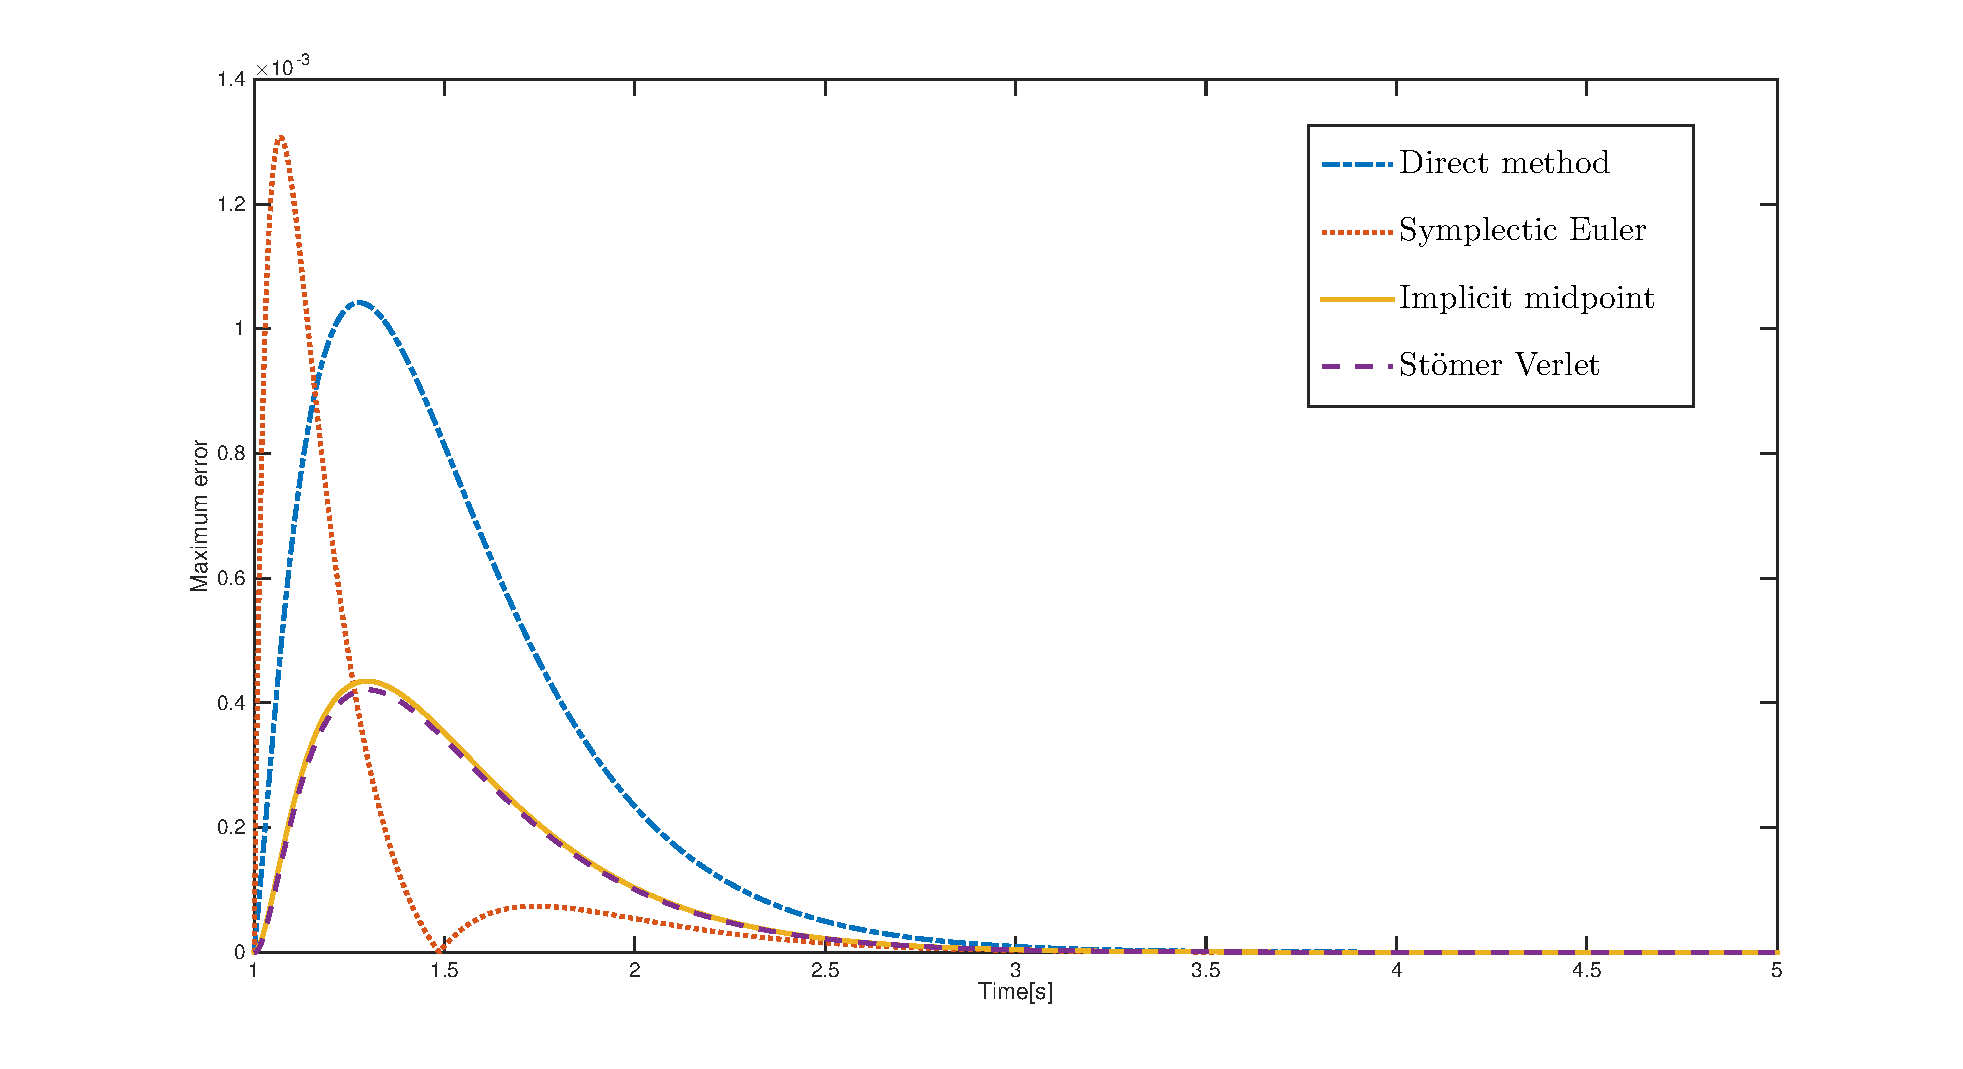
\includegraphics[width=0.8\textwidth]{02/Fig2.pdf}
    \caption{表中展示了4种方法在 $[0,5]$ 区间的误差无穷范数的变化结果}
    \label{fig:err1}
\end{figure}


\subsection*{算例 2}
在此例子中,取方程中的参数为 $a = 100, b
=-100\pi$ 和 $k =30\pi$. 并进行和算例 1 中同样的计算.
精确解为 $e^{-10\pi t}\sin(\pi t)$. 初值和边值条件分别为
\begin{equation*}
\begin{aligned}
w(x,0)&=\sin(\pi x),\\
w_t(x,0)&=-10 \pi \sin(\pi x),
\end{aligned}
\end{equation*}
和
\begin{equation*}
\begin{aligned}
w(0,t)&=0,\\
w(1,t)&=0.
\end{aligned}
\end{equation*}

通过变换 $w=e^{-15\pi t}u$, 得到方程 \eqref{eq:kg}, 其中初值条件为
\begin{equation*}
\begin{aligned}
u(x,0)&=\sin(\pi x),\\
u_t(x,0)&=5\pi \sin(\pi x),
\end{aligned}
\end{equation*}
边值条件为
\begin{equation*}
\begin{aligned}
u(0,t)&=0,\\
u_t(1,t)&=0.
\end{aligned}
\end{equation*}

数值结果如下.

\textbf{$\Delta x$ 的阶}

首先,为了检验 $\Delta x$ 的阶, 固定比较小的 $\Delta
t$, 通过相应地变化 $\Delta x$ 来得到. 取 $\Delta t = 0.0001$, 和 $T
= 1$, 结果在表 \ref{tab:dx2} 中给出,可以看到隐式中点法和 St\"{o}rmer-Verlet 方法为二阶.

\begin{table}[h]
  \centering
\caption{表中比较了随 $\Delta x$ 的变化,误差的无穷范数变化情况,其中 $\Delta t=0.0001$ 和 $T=1$}
\begin{tabularx}{\linewidth}{XXXXX}
 \toprule[1.5pt]
$\Delta x$ &直接方法 & 辛欧拉 & 隐式中点 & St\"{o}rmer-Verlet\\
 \midrule[1pt]
 0.1 & 0.6487 & 0.0013 & 0.0013 & 0.0013\\
 0.05 & 0.6496 & 2.7325e-04 & 3.3279e-04 & 3.3271e-04\\
 0.025 & 0.6498 & 6.2785e-05 & 8.3249e-05 & 8.3174e-05\\
 0.0125 & 0.6499 & 8.6850e-05 & 2.0839e-05 & 2.0764e-05\\
 0.00625 & 0.6499 & 9.5203e-05 & 5.2348e-06 & 5.1600e-06\\
 \bottomrule[1.5pt]
\end{tabularx}
  \label{tab:dx2}
\end{table}

\textbf{$\Delta t$ 的阶}

其次,固定较小地 $\Delta x = 0.01$, 相应地变化 $\Delta t$, 得到表 \ref{tab:dt2} 的结果,可以看到直接方法为一阶.

\begin{table}[h]
  \centering
\caption{表中比较了随 $\Delta t$ 的变化,误差的无穷范数变化情况,其中 $\Delta x=0.01$ 和 $T=2$}
\begin{tabularx}{\linewidth}{XXXXX}
 \toprule[1.5pt]
 $\Delta t$ &直接方法 & 辛欧拉 & 隐式中点 & St\"{o}rmer-Verlet\\
 \midrule[1pt]
 0.001 & 0.6467 & 9.7975e-04 & 1.6714e-05 & 9.4887e-06 \\
 0.0005 & 0.6485 & 4.8457e-04 & 1.4153e-05 & 1.2295e-05 \\
 0.00025 & 0.6493 & 2.3809e-04 & 1.3524e-05 & 1.3057e-05 \\
 0.000125 & 0.6498 & 1.1523e-04 & 1.3368e-05 & 1.3251e-05 \\
 0.0000625 & 0.6500 & 5.4100e-05 & 1.3329e-05 & 1.3299e-05 \\
 \bottomrule[1.5pt]
\end{tabularx}
  \label{tab:dt2}
\end{table}

\textbf{长时间性质}

最后,固定 $\Delta x = 0.01$ 和 $\Delta t = 0.001$, 改变时间区间 $T$ 来查看长时间性质,得到表 \ref{tab:t2} 中的结果,可以看到所有方法长时间性质良好.

\begin{table}[h]
  \centering
\caption{表中比较了随 $T$ 的变化,误差的无穷范数变化情况,其中 $\Delta x=0.01$ 和 $\Delta t=0.001$}
\begin{tabularx}{\linewidth}{XXXXX}
 \toprule[1.5pt]
 $T$ &直接方法 & 辛欧拉 & 隐式中点 & St\"{o}rmer-Verlet\\
 \midrule[1pt]
 1 & 0.6467 & 9.7975e-04 & 1.6714e-05 & 9.4887e-06 \\
 10 & 0.6467 & 9.7975e-04 & 1.6714e-05 & 9.4887e-06 \\
 100 & 0.6467 & 9.7975e-04 & 1.6714e-05 & 9.4887e-06 \\
 1000 & 0.6467 & 9.7975e-04 & 1.6714e-05 & 9.4887e-06 \\
 \bottomrule[1.5pt]
\end{tabularx}
  \label{tab:t2}
\end{table}

\subsection*{算例 3}
在此例子中,我们求解二维的电报方程,
\begin{equation*}
\frac{\partial ^2 w}{\partial t^2}+8\pi \frac{\partial w}{\partial
t}=4 (\frac{\partial ^2 w}{\partial x^2} + \frac{\partial ^2
w}{\partial y^2}) -3\pi^2 w.
\end{equation*}
精确解为 $w(x,t) = e^{-\pi t}sin(\pi x)sin(\pi y)$. 初值和边值条件能够相应地得到,这里不再赘述.

\textbf{$\Delta x$ 的阶}

首先,固定 $\Delta t$, 相应地变化 $\Delta x$, 并取
$\Delta t = 0.0001$ 和 $T = 1$. 得到表 \ref{tab:dx3} 中的结果,可以看到隐式中点法和 St\"{o}rmer-Verlet 方法为二阶.

\begin{table}[h!]
  \centering
\caption{表中比较了随 $\Delta x$ 的变化,误差的无穷范数变化情况,其中 $\Delta t=0.001$ 和 $T=2$}
\begin{tabularx}{\linewidth}{XXXXX}
 \toprule[1.5pt]
 $\Delta x$ &直接方法 & 辛欧拉 & 隐式中点 & St\"{o}rmer-Verlet\\
 \midrule[1pt]
 0.1 & 0.8252 & 0.0018 & 0.0017 & 0.0017\\
 0.05 & 0.8301 & 5.0684e-04 & 4.2688e-04 & 4.2674e-04\\
 0.025 & 0.8314 & 2.0812e-04 & 1.0680e-04 & 1.0667e-04\\
 0.0125 & 0.8317 & 1.5813e-04 & 2.6763e-05 & 2.6625e-05\\
 \bottomrule[1.5pt]
\end{tabularx}
  \label{tab:dx3}
\end{table}

\textbf{$\Delta t$ 的阶}

其次,固定一个较小的 $\Delta x = 0.01$, 相应地变化 $\Delta t$, 得到了表 \ref{tab:dt3} 的结果,可以看到辛欧拉方法为一阶.

\begin{table}[h]
  \centering
\caption{表中比较了随 $\Delta t$ 的变化,误差的无穷范数变化情况,其中 $\Delta x=0.01$ 和 $T=1$}
\begin{tabularx}{\linewidth}{XXXXX}
 \toprule[1.5pt]
 $\Delta t$ &直接方法 & 辛欧拉 & 隐式中点 & St\"{o}rmer-Verlet\\
 \midrule[1pt]
 0.001 & 0.8317 & 0.0015 & 2.5175e-05 & 1.1497e-05 \\
 0.0005 & 0.8317 & 7.3588e-04 & 1.9097e-05 & 1.5646e-05 \\
 0.00025 & 0.8317 & 3.7202e-04 & 1.7581e-05 & 3.0713e-05 \\
 0.000125 & 0.8317 & 1.8992e-04 & 1.7203e-05 & 8.5729e-06 \\
 \bottomrule[1.5pt]
\end{tabularx}
  \label{tab:dt3}
\end{table}

\textbf{长时间性质}

最后,固定 $\Delta x = 0.1$ 和 $\Delta t = 0.001$, 通过变化求解区间长度 $T$ 来查看长时间性质,得到表 \ref{tab:t3} 的结果,可以看到所有方法长时间性质良好.

\begin{table}[h]
  \centering
\caption{表中比较了随 $T$ 的变化,误差的无穷范数变化情况,其中 $\Delta x=0.1$ 和 $\Delta t=0.001$}
\begin{tabularx}{\linewidth}{XXXXX}
 \toprule[1.5pt]
 $T$ &直接方法 & 辛欧拉 & 隐式中点 & St\"{o}rmer-Verlet\\
 \midrule[1pt]
 1 & 0.8252 & 0.0026 & 0.0017 & 0.0017 \\
 10 & 0.8599 & 0.0026 & 0.0017 & 0.0017 \\
 100 & 0.8599 & 0.0026 & 0.0017 & 0.0017 \\
 1000 & 0.8599 & 0.0026 & 0.0017 & 0.0017 \\
 \bottomrule[1.5pt]
\end{tabularx}
  \label{tab:t3}
\end{table}

\subsection{结果分析}
\esubsection{Analysis of Results}

根据数值实验的结果,可以得到如下结论.首先,数值结果的全局误差由 CFL 条件和步长来制约.其次,由于全局误差界为 $O(\Delta x^2+ \Delta t^k)$, 能够在数值解上近似地看出阶条件.在这里,可以知道数值结果符合阶条件,和理论值相匹配.第三,长时间性质能够很好地保持.

此外,对于过长时间的计算是不必要的,因为该问题在一定长的时间后数值衰减得很小,超过机器误差的最小值,故不做过长计算.

\begin{remark}
{\rm 注意到,这里我们没有对哈密尔顿量的结果进行比较,因为变化之后,数值上比较大,哈密尔顿量的变化会很灵敏.此时,可能要求去比较相对误差,然而该系统的哈密尔顿量保持在常值 $0$, 又使得我们无法使用相对误差作为衡量.因此可能需要一个更精妙的数值格式来保持,或者寻找一个新的评价标准来分析该方法的效果.然而,根据误差结果,我们有理由相信算法的有效性.}
\end{remark}

\section{小结}\label{sec:02conclusion}
\esection{Brief Summary}
在本章中,提出了一种新的求解带有齐次边界条件的电报方程的方法.该方法有效地利用了一个将非哈密尔顿系统化为哈密尔顿系统的变换,结合了辛方法的特性,得到了较好的效果.我们讨论了该算法的阶条件,~CFL 条件,长时间性质和局限性.在空间离散上取了二阶的离散格式,得到了 $O(\Delta x^2+ \Delta
t^k)$ 的误差界. 该方法的优势在于利用了辛方法长时间求解的好的性质.另外, 我们的解可以看作一个很优美的哈密尔顿系统乘以一个函数的结果.我们方法的基本思想是先变换,再求解,再逆变换,和傅立叶变换的思想比较类似.数值结果展示了阶条件,算法的有效性和长时间性质.该方法不局限于使用文中提及的辛格式,其他合适的辛格式也可以使用进来.非齐次的问题,需要增加两个分量来求解,该部分在文中注解部分有所提及.
